\documentclass[11pt,a4paper]{article}
\usepackage[margin=0.92in]{geometry}
\usepackage{amsmath,amssymb,booktabs,graphicx,array,float}
\usepackage[colorlinks=true,linkcolor=blue,urlcolor=blue,citecolor=blue]{hyperref}
\usepackage{microtype}
\graphicspath{{docs/figures/}{results/analysis/figures/}}
\newcommand{\R}{\mathbb{R}}
\newcommand{\norm}[1]{\left\lVert #1\right\rVert}
\newcommand{\dd}{\,\mathrm{d}}
\title{From Residual Direction to Reliable Trajectories:\\A Study of Physics-Informed Neural Networks for Lorenz-63}
\author{Differential Equations Semester Project\\Continuation of the submitted project report}
\date{22 November 2026}
\begin{document}
\maketitle
\begin{abstract}
The project asks whether the direction of a physics-informed neural network (PINN) residual, in addition to its magnitude, predicts later trajectory error in a chaotic ordinary differential equation. Turinici's regime-aware time-weighting paper motivated the question: its scalar error bound prioritizes when residuals occur but cannot describe their orientation. A linear saddle verifies that equal-size residuals can have very different effects. We then test two reference-derived expanding directions on Lorenz-63 PINNs with a fixed, held-out prediction rule. Neither direction passes that rule in the original 40 runs, nor in 40 fresh runs of a more accurate sequential PINN. A sparse-residual interpolation and trailing-average study finds exploratory short-horizon predictive value from residual history. Model development improves a two-time-unit pilot from median error 6.052 to 0.0259, but fresh validation shows only 30 of 40 sequential runs remain below error 1 throughout. We also port the reference paper's adaptive time-weighting rule, checking both its equation and source-code time scales. Neither improves our matched global pilot or one-seed eight-window sequential comparison. Full reference-based tangent amplification adds held-out predictive information at longer horizons; it is an oracle diagnostic. The final conclusion is a bounded negative result for one-vector pointwise alignment, accompanied by a useful sequential model and a clearer account of which residual information matters.
\end{abstract}
\tableofcontents
\clearpage

\section{Original question, objective, and scope}
Our submitted report, \emph{Project Report -- Differential Equations -- 2} \cite{submitted}, proposed studying the relation between differential-equation residuals and future PINN error. The goal was not simply to reduce a loss: it was to understand whether a residual's \emph{direction} identifies the part of a local defect that chaotic dynamics will amplify. A useful answer could eventually guide diagnostics or a directional training loss.

The central hypothesis was: at fixed residual magnitude, a residual aligned with a locally expanding direction should produce or predict greater later trajectory error than one aligned with a contracting direction. The precise empirical question is narrower. Given an already trained Lorenz PINN, does a one-time alignment score improve prediction of \emph{total future error} on an initial condition withheld from regression fitting, beyond knowledge of residual magnitude? We separately consider a finite-time singular direction and a backward Lyapunov direction. This distinction matters because Lorenz's Jacobian is nonnormal and the two directions need not coincide.

We proceeded in four stages: derive the mechanism in a solvable linear system; construct trusted Lorenz references and tangent directions; test the prespecified hypothesis on standard PINNs; then explore residual history and improve the PINN enough to revisit the question over a longer interval. The main result is a scientific outcome even though the initial hypothesis was unsupported: it identifies a limit of a plausible pointwise diagnostic and measures the practical improvement and remaining failures of the revised solver.

\section{Reference paper: what it establishes and what it suggested}
\subsection{PINN residual and time-weighted training}
Turinici's \emph{Regime-Aware Time Weighting for Physics-Informed Neural Networks}, arXiv:2407.21642v2 \cite{turinici}, considers a time-dependent equation $\partial_t u=\mathcal G_t(u)$ and a candidate $U_\theta$. Its equation residual $w=\partial_t U_\theta-\mathcal G_t(U_\theta)$ is the forcing that makes the candidate satisfy a perturbed equation exactly. A time-weighted squared-residual objective is
\begin{equation}\label{eq:paperloss}
 \mathcal L_{\rho}(\theta)=\int_0^T\rho(t)\norm{w(t)}^2\dd t,
 \qquad \rho(t)\geq0,\quad\int_0^T\rho(t)\dd t=1.
\end{equation}
For an ODE the spatial integral of the general paper disappears. Time weighting concerns \emph{when} the PINN violates the equation. Our original training objective, described below, used a uniform residual term and a soft initial-condition penalty; it was not an implementation of Eq.~\eqref{eq:paperloss} with the paper's adaptive weight.

\subsection{The error bound and the paper's optimal density}
The paper assumes an exact initial condition and a one-sided growth-rate bound $\lambda(t)$ for the difference between the exact and candidate vector fields. For its sign convention $e_p=u-U_\theta$, the assumption and terminal-error bound are
\begin{align}
\frac{\langle\mathcal G_t(u)-\mathcal G_t(U_\theta),u-U_\theta\rangle}{\norm{u-U_\theta}^2}&\leq\lambda(t),\label{eq:onesided}\\
\norm{e_p(T)}&\leq\int_0^T\exp\!\left(\int_t^T\lambda(s)\dd s\right)\norm{w(t)}\dd t.\label{eq:bound}
\end{align}
To see the logic, differentiating $\norm{e_p}^2/2$, applying Eq.~\eqref{eq:onesided} and Cauchy--Schwarz gives $\frac{\dd}{\dd t}\norm{e_p}\leq\lambda\norm{e_p}+\norm{w}$. Integrating the resulting scalar inequality gives Eq.~\eqref{eq:bound}. With nonzero initial error the bound gains the term $\exp(\int_0^T\lambda)\norm{e_p(0)}$; this matters for our original soft-IC PINN.

The paper fixes a budget $\int_0^T\rho(t)\norm{w(t)}^2\dd t\leq C_p$ and minimizes the worst value of the right-hand side of Eq.~\eqref{eq:bound} over possible bounded residuals. Put $\Lambda(t)=\exp[-\int_0^t\lambda(s)\dd s]$. Then Cauchy--Schwarz gives
\begin{equation}
\left(\int_0^T\Lambda\norm{w}\dd t\right)^2
\leq C_p\int_0^T\frac{\Lambda(t)^2}{\rho(t)}\dd t,
\qquad
\int_0^T\frac{\Lambda^2}{\rho}\dd t\geq\left(\int_0^T\Lambda\dd t\right)^2.
\end{equation}
Equality in the second inequality yields the paper's density
\begin{equation}\label{eq:rho}
\rho_{\rm opt}(t)=\frac{\exp[-\int_0^t\lambda(s)\dd s]}
{\int_0^T\exp[-\int_0^q\lambda(s)\dd s]\dd q}.
\end{equation}
For positive growth the density emphasizes earlier times; for negative growth it can emphasize later times. This is an optimum of the stated \emph{minimax bound under a fixed weighted-loss budget}, not a guarantee that finite neural-network training will yield the smallest actual error. The paper estimates $\lambda$ during training approximately by replacing the unavailable exact state with zero:
\begin{equation}\label{eq:lambdaest}
\lambda_n(t)\sim
\frac{\langle\mathcal G_t(U_{\theta_n})-\mathcal G_t(0),U_{\theta_n}\rangle}
{\norm{U_{\theta_n}}^2}.
\end{equation}
This is a practical growth proxy, not a precisely measured largest Lyapunov exponent. The paper tests its training method on Lorenz and Burgers' equation. We learned two things from it: residuals must be interpreted through dynamics, and their timing is important. Our extension asked whether the scalar norm and scalar growth bound conceal useful \emph{directional} information. We do not claim to reproduce its adaptive weighting experiment.

\section{Our mathematical model and initial hypothesis}
\subsection{Lorenz-63, residuals, and exact error dynamics}
Let $X=(x,y,z)^\top$ and
\begin{equation}\label{eq:lorenz}
\dot X=f(X)=\begin{pmatrix}\sigma(y-x)\\x(\rho-z)-y\\xy-\beta z\end{pmatrix},
\quad (\sigma,\rho,\beta)=(10,28,8/3).
\end{equation}
For a PINN trajectory $\widehat X_\theta$, define the residual $r=\dot{\widehat X}_\theta-f(\widehat X_\theta)$ and error $e=\widehat X_\theta-X$. The exact identity is
\begin{equation}\label{eq:exacterror}
\dot e=f(\widehat X_\theta)-f(X)+r.
\end{equation}
The Lorenz Jacobian is
\begin{equation}\label{eq:jac}
J(X)=\begin{pmatrix}-\sigma&\sigma&0\\\rho-z&-1&-x\\y&x&-\beta\end{pmatrix}.
\end{equation}
When $e$ is small, $f(X+e)-f(X)=J(X)e+O(\norm e^2)$. If $\Phi(t,s)$ satisfies $\partial_t\Phi(t,s)=J(X(t))\Phi(t,s)$ and $\Phi(s,s)=I$, variation of constants gives the \emph{linearized} reconstruction
\begin{equation}\label{eq:duhamel}
e(t)\approx\Phi(t,0)e(0)+\int_0^t\Phi(t,s)r(s)\dd s.
\end{equation}
The first term is inherited initial-condition error; the integral combines residual direction, magnitude, timing, and cancellation. For nonlinear Lorenz, Eq.~\eqref{eq:duhamel} is an approximation, not the exact identity \eqref{eq:exacterror}. It also explains why $r(t)$ at a single instant need not predict \emph{total} error at $t+\Delta$: much of that error may already exist.

\subsection{Sanity check: equal-size residuals with unequal effects}
For the saddle $\dot Z=AZ$, $A=\operatorname{diag}(1,-1)$, a constant residual $r=\varepsilon(1,0)^\top$ acting from zero error produces $e(t)=\varepsilon(e^t-1,0)^\top$. The equal-norm residual $r=\varepsilon(0,1)^\top$ produces $e(t)=\varepsilon(0,1-e^{-t})^\top$. At $t=5$ the error magnitudes differ by $e^5\simeq148$ despite identical $\norm r=\varepsilon$. The experiment reproduced these analytic values \cite{phase0}. For a short horizon the difference is small: both first grow approximately $\varepsilon\Delta$. This toy proves the mechanism can exist; it does not imply that trained Lorenz PINNs supply enough variation in direction to detect it.

\subsection{Which expanding direction?}
We compute the tangent propagator along each trusted reference. The leading backward Lyapunov vector $b_1(t)$ comes from repeated forward propagation and QR reorthogonalization, $\Phi(t_{i+1},t_i)Q_i=Q_{i+1}R_i$. It summarizes the direction into which \emph{past} perturbations have aligned. The leading right singular vector $s_1(t;\Delta)$ of $\Phi(t+\Delta,t)=U\Sigma V^\top$ maximizes growth over exactly the \emph{future} horizon $\Delta$. In a nonnormal system these vectors differ; the finite-time singular vector is the more direct candidate for a newly introduced residual. Neither candidate is computed from the PINN alone: both use the exact-reference trajectory and are therefore oracle directions in this diagnostic study.

At each predictor time define
\begin{equation}\label{eq:features}
R=\norm{r(t)},\quad A_u=\frac{|r(t)^\top u(t)|}{R+10^{-12}},\quad
R_u=|r^\top u|,\quad R_\perp=\norm{r-(r^\top u)u},\quad
R_\Phi=\norm{\Phi(t+\Delta,t)r(t)}.
\end{equation}
$R_\Phi$ uses all singular directions and their gains: if $r=\sum_i\alpha_i s_i$, then $R_\Phi^2=\sum_i\sigma_i^2\alpha_i^2$. An alignment with just $s_1$ omits the other coefficients and gains. The oracle feature is useful for testing the mechanism but unavailable without the true trajectory.

\section{Experimental design and original PINN}
\subsection{Reference construction and tangent checks}
A long Lorenz trajectory starts from $(1,1,1)$; the first 100 time units are discarded. Nine windows start 20 units apart at long-run times $130+20k$, $k=0,\ldots,8$. Window 0 is reserved for pilot choices; windows 1--8 provide eight initial conditions. Each has a 30-unit preceding trajectory for convergence of $b_1$. A fresh DOP853 solve on each window, relative tolerance $10^{-12}$ and absolute tolerance $10^{-14}$, is sampled at spacing 0.002. A stricter DOP853 solve and LSODA cross-check establish a reference trust horizon beyond the PINN intervals. For the original windows the minimum $10^{-8}$ trust horizon was about 5.8; the fresh set's minimum was 5.83, both beyond the final $T=2$ test. Tangent matrices were integrated along the dense reference, and QR-derived Lyapunov exponents on the original long run were approximately $(0.924,-0.025,-14.566)$; the fresh run gave $(0.9015,-0.0023,-14.5658)$. Their sum agrees with $\mathrm{tr}J=-(\sigma+1+\beta)=-13.6667$ \cite{phase2,phase3,validation}.

\subsection{Original network and actual training loss}
The baseline PINN has four hidden layers of width 64 with $\tanh$ activations. For $t\in[0,T]$, $\tau=2t/T-1$ and $\widehat X_\theta(t)=m+10N_\theta(\tau)$, $m=(0,0,25)^\top$. Automatic differentiation supplies $\dot{\widehat X}_\theta$ and the three-component residual. The original objective was
\begin{equation}\label{eq:softloss}
L_{\rm soft}(\theta)=\underbrace{\frac1N\sum_{i=1}^N\norm{\dot{\widehat X}_\theta(t_i)-f(\widehat X_\theta(t_i))}^2}_{L_{\rm ODE}}
+\lambda_{\rm IC}\underbrace{\norm{\widehat X_\theta(0)-X_0}^2}_{L_{\rm IC}},
\quad N=1024,\quad\lambda_{\rm IC}=100.
\end{equation}
The 1024 collocation times are stratified samples redrawn each Adam step. There are 20,000 updates and an exponential learning-rate schedule from $10^{-3}$ to $10^{-5}$. During the first 60\% of updates a time curriculum expands the collocation interval from 0.25 to $T$; afterward the full interval is sampled. Training uses float32, while saved residuals are recomputed in float64 \cite{phase4}.

The first global $T\geq2$ pilots sometimes converged near the invariant Lorenz $z$-axis trajectory: a small residual could coexist with a large trajectory error because a local defect near the initial time pushed the network to another valid solution. The pilot therefore selected $T=1$ for the primary test. The stated pilot rule would literally have chosen $\lambda_{\rm IC}=10$ by an average over failed long windows, but the main study used 100 because it was much more accurate at the only workable $T=1$. We report that deviation; a full 40-run $\lambda_{\rm IC}=10$ sensitivity study gave the same hypothesis verdict.

\subsection{Prespecified prediction test}
For $\Delta\in\{0.05,0.1,0.25,0.5,1\}$, the primary target is $E_\Delta(t)=\norm{e(t+\Delta)}$; the secondary target removes linearly inherited error, $N_\Delta(t)=\norm{e(t+\Delta)-\Phi(t+\Delta,t)e(t)}$. On a 0.01 statistics grid we fit ordinary least squares to $y=\log E_\Delta$:
\begin{align}
M_0:&\quad y=a+b\log R,\label{eq:m0}\\
M_1(u):&\quad y=a+b\log R+cA_u,\qquad u\in\{b_1,s_1\}.\label{eq:m1}
\end{align}
Other planned features include $\log R_u$ and the oracle $\log(R_\Phi/R)$. Every fit uses seven initial-condition windows and predicts the eighth; we pool the eight held-out folds and compute $R^2=1-\sum_i(y_i-\widehat y_i)^2/\sum_i(y_i-\bar y)^2$. The decisive quantity is $\Delta R^2=R^2(M_1)-R^2(M_0)$. Uncertainty in the original study comes from 2000 cluster resamples of runs applied to out-of-fold predictions, not from treating individual time points as independent.

The rule, written before seeing the original 40-run outcome, required at least three horizons to show $\Delta R^2\geq0.02$ with a positive 95\% interval, a positive fitted alignment coefficient, gain beyond the 95th percentile of 20 random-direction and 20 time-shuffled controls, and a positive fixed-magnitude alignment effect with a positive interval. We also examined contracting and flow directions, the secondary target, and samples with current and future error below 1. At $T=1$, $\Delta=1$ leaves only $t=0$ and is unusable, so the rule applies to four horizons. The directional training-loss phase was conditional on this rule passing; it was not run \cite{plan,results}.

\section{Original test: what happened and why the hypothesis failed empirically}
All 40 baseline runs (eight windows, five seeds) were retained. Table~\ref{tab:original} gives held-out results. Neither $b_1$ nor $s_1$ passes the first part of the fixed rule at any usable horizon. At $\Delta=0.5$, $s_1$ has a positive interval but gain $0.017<0.02$. The oracle feature is secondary: it has positive intervals at 0.25 and 0.5, but needs the reference propagator.
\begin{table}[H]\centering\small
\caption{Original $T=1$ PINNs: pooled held-out $R^2$ for residual magnitude and gains from adding one direction or full amplification. Brackets are reported 95\% run-bootstrap intervals.}\label{tab:original}
\begin{tabular}{@{}ccccc@{}}\toprule
$\Delta$ & $R^2(M_0)$ & $\Delta R^2(b_1)$ & $\Delta R^2(s_1)$ & $\Delta R^2(\Phi)$\\\midrule
0.05 & $-0.20$ & $+.003\;[-.031,.026]$ & $+.046\;[-.007,.094]$ & $+.019$\\
0.10 & $-0.13$ & $+.010\;[-.030,.036]$ & $+.031\;[-.036,.087]$ & $+.026$\\
0.25 & $+.27$ & $+.020\;[-.032,.055]$ & $+.025\;[-.038,.078]$ & $+.067\;[.011,.120]$\\
0.50 & $+.74$ & $-.008\;[-.026,.003]$ & $+.017\;[.002,.033]$ & $+.056\;[.040,.087]$\\\bottomrule
\end{tabular}
\end{table}
\begin{figure}[H]\centering
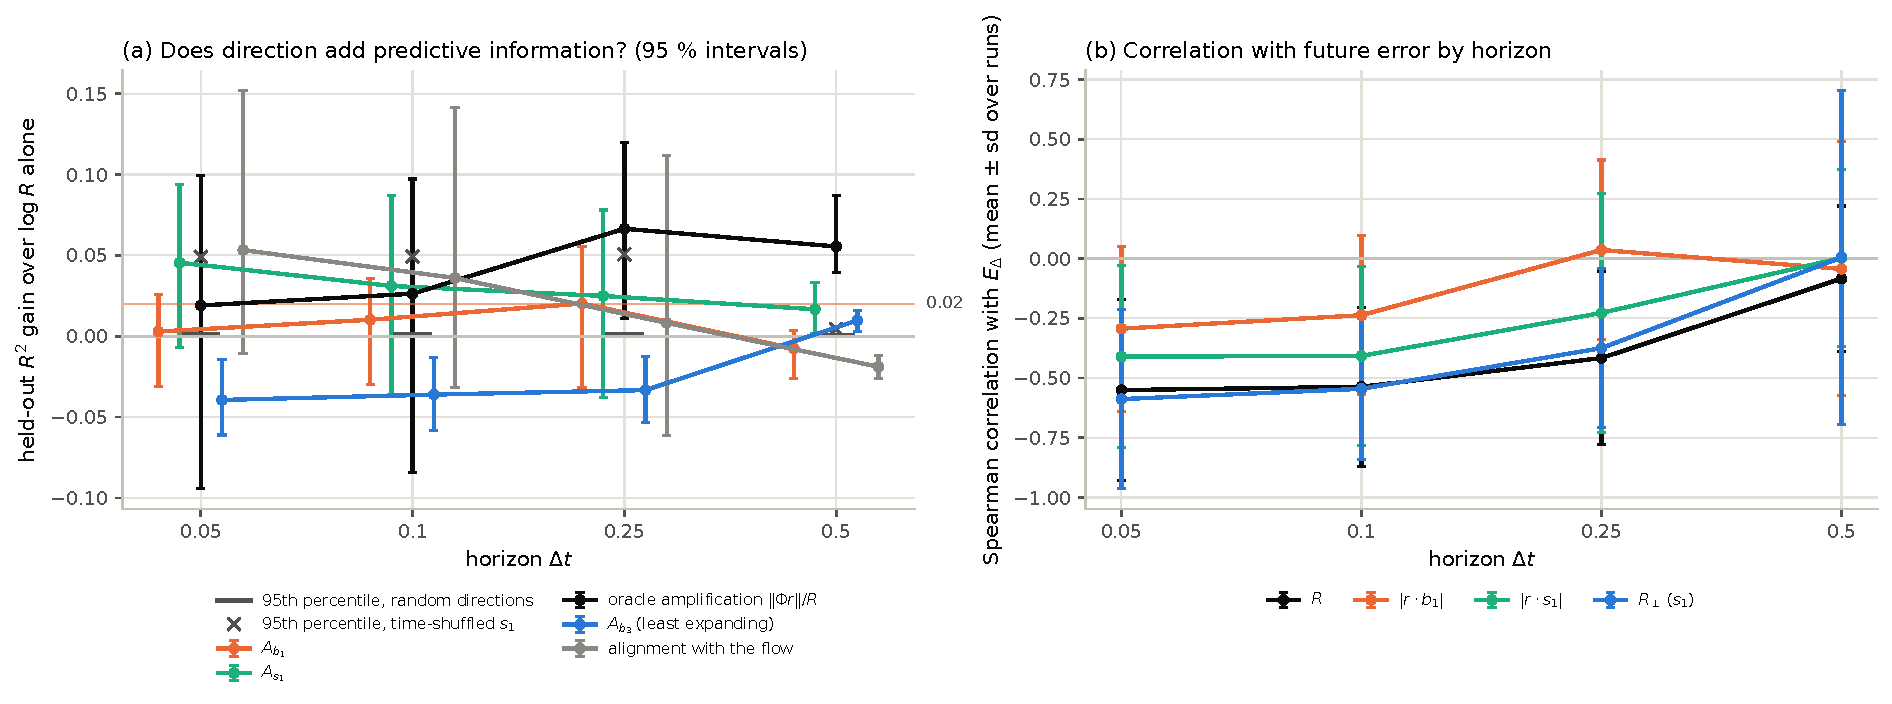
\includegraphics[width=.86\linewidth]{fig04_horizon_summary.pdf}
\caption{Original planned held-out horizon analysis, produced by this repository. The decision concerns gains beyond residual magnitude, not the training loss.}\label{fig:original}
\end{figure}
The null conclusion persists in the full $\lambda_{\rm IC}=10$ sensitivity (40 runs), the smaller float64 set (eight runs), the near-linear subset, and the created-error target \cite{results}. A within-run fixed-magnitude association exists at short horizons, but random or time-shuffled controls and the neutral flow direction can have comparable effects; it does not generalize to held-out initial conditions.

Two observed features help interpret the result without proving a unique cause. First, trained residuals are already strongly aligned with $s_1$ (median alignment 0.96 at $\Delta=0.25$), leaving little contrast between otherwise equal-size residuals. Second, the total error at a future time contains earlier, inherited error; a current residual may be small after the trajectory has drifted. In the original smooth models, Eq.~\eqref{eq:duhamel}'s median relative reconstruction mismatch was about 6\%, and initial-condition error accounted for about 3\% on average. Thus the residual-forcing picture is useful, but a single pointwise projection discards history and much of the propagator. The study does \emph{not} demonstrate that residual direction is physically irrelevant or that any one proposed mechanism alone caused the null prediction result.

\section{Exploratory continuation: sparse residual interpolation}
The submitted report suggested reconstructing residuals from sparse samples and using their history. We rebuilt all 40 original PINN arrays because the saved summary JSON did not contain the required trajectories. Residual vectors were sampled every 0.05 time units, compared with the dense 0.002 grid. Linear interpolation reconstructs $\widetilde r_{\rm lin}(s)$ between consecutive knots; a sample-and-hold version and a simple average of knot magnitudes provide controls. At a prediction knot $t$ with a complete preceding interval of width $w\in\{0.1,0.25\}$, the history feature is
\begin{equation}\label{eq:trailing}
H_w(t)=\frac1w\int_{t-w}^{t}\norm{\widetilde r(s)}\dd s.
\end{equation}
The held-out regression adds $\log H_w$ to a baseline using pointwise $\log\norm{\widetilde r_{\rm lin}(t)}$ and normalized time. Evaluation is only at observed knots, so the integral uses no residual measured after prediction time. An initial analysis at intermediate fine-grid times accidentally allowed linear interpolation to use a future knot; its predictive scores were invalidated and replaced by this causal-at-evaluation-time design \cite{interpolation}.

For width 0.25 the linear-history feature increased held-out $R^2$ over pointwise magnitude plus time by $+0.474$, $+0.472$, and $+0.312$ for horizons 0.05, 0.1, and 0.25. The direct gain over sample-and-hold was much smaller: $+0.058$, $+0.055$, and $+0.052$. A post-result box control averaging observed knot magnitudes including the current knot gave a similar baseline; the linear gain over it was about $+0.05$ to $+0.06$ at horizons 0.1 and 0.25. At horizon 0.5 the gain of any trailing average over the pointwise-plus-time baseline was uncertain. Linear reconstruction also recovered dense trailing averages more accurately than hold (relative absolute error 0.071 versus 0.079 for width 0.25) \cite{interpolation}.
\begin{table}[H]\centering\small
\caption{Exploratory sparse-residual history test at trailing width $w=0.25$. Gains are held-out $R^2$ changes over pointwise residual magnitude plus time, on the same sampled-knot prediction times. The box control averages observed knot magnitudes, including the current knot.}\label{tab:interpolation}
\begin{tabular}{@{}ccccc@{}}\toprule
Future horizon & Baseline $R^2$ & Linear gain & Hold gain & Box gain\\\midrule
0.05 & 0.197 & $+0.474$ & $+0.416$ & $+0.411$\\
0.10 & 0.279 & $+0.472$ & $+0.417$ & $+0.412$\\
0.25 & 0.568 & $+0.312$ & $+0.260$ & $+0.261$\\
0.50 & 0.817 & $+0.043$ & $-0.002$ & $\approx0$\\\bottomrule
\end{tabular}
\end{table}
\begin{figure}[H]\centering
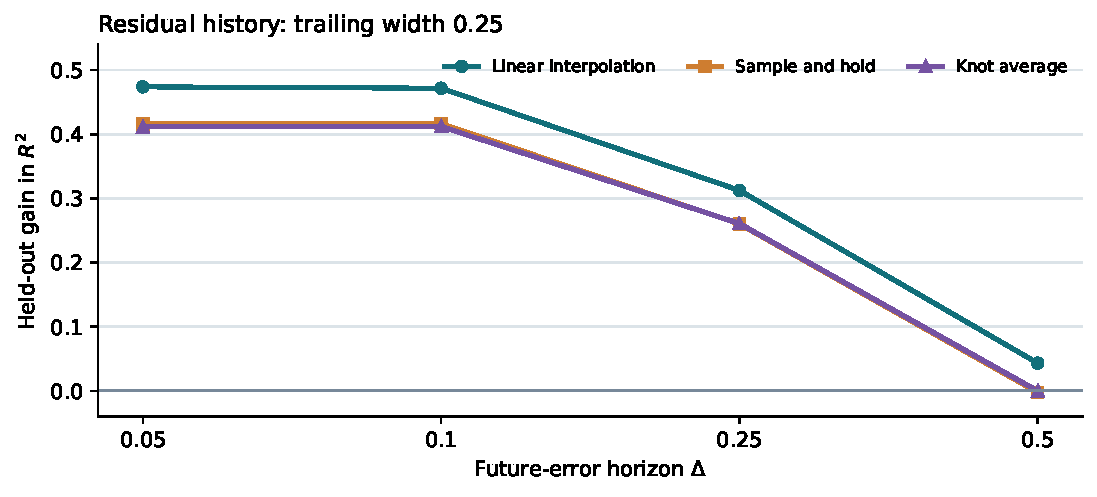
\includegraphics[width=.82\linewidth]{report_interpolation_gains.pdf}
\caption{Exploratory held-out prediction gains at trailing width $0.25$, generated from the corrected sampled-knot metrics. All three methods include residual history; the smaller gap between linear reconstruction and the two simpler controls is the interpolation-specific effect. The gain at horizon $0.5$ over the pointwise baseline is uncertain.}\label{fig:interpolation}
\end{figure}
At the other explored width, $w=0.10$, linear gains over the same pointwise baseline were $+0.288$, $+0.295$, $+0.216$, and $+0.049$ in increasing horizon order. Linear interpolation better reconstructs the dense history feature than hold, but predictive gains depend on the regression target, window width, and control. For example, the interval for the $w=0.10$, $\Delta=0.05$ linear-minus-box gain includes zero; we therefore do not generalize the modest interpolation-specific effect to every horizon and width. The corrected analysis uses eight window clusters and resamples held-out predictions without refitting in each bootstrap draw, so its intervals describe this dataset rather than a confirmatory guarantee.

The useful signal is principally \emph{recent residual magnitude}; interpolation contributes a smaller, exploratory increment. These widths, horizons, and the box control were explored after the original study, and there are only eight independent initial-condition windows. The interpolation analysis used a restricted prediction-time subset and a time-adjusted baseline, so its $R^2$ values are not directly comparable to Table~\ref{tab:original}. It did not improve the PINN trajectory by changing training. Gaussian-process smoothing and a held-out Duhamel-integrated predictor remain untested proposals. The adaptive time-weighting experiment is reported separately in Section~\ref{sec:adaptive}.

\section{Improving the trajectory model and revisiting the question}
\subsection{Hard initial condition, early weighting, and optimization}
The global $T=2$ soft-IC pilot had median trajectory error 17.476 despite median residual magnitude 0.083. We first enforced the initial state by writing
\begin{equation}\label{eq:hardic}
\widehat X_\theta(t)=X_0+\frac{t}{T}\bigl(g_\theta(t)-X_0\bigr),
\qquad \widehat X_\theta(0)=X_0,
\end{equation}
with $g_\theta$ a scaled neural-network output. Its training loss becomes only $L_{\rm ODE}=N^{-1}\sum_i\norm{r(t_i)}^2$. On the same pilot window, the median error fell to 6.052, still too large. We then tried a simple early-time weight,
\begin{equation}\label{eq:earlyweight}
L_{\rm early}(\theta)=\frac{\sum_i[1+9(1-t_i/T)]\norm{r(t_i)}^2}
{\sum_i[1+9(1-t_i/T)]}.
\end{equation}
Its pilot median error was 6.036; the fraction of points with error below 1 rose only from 11.3\% to 12.6\%. This fixed linear weight is \emph{not} Turinici's adaptive density \eqref{eq:rho}. Refining the hard-IC model with 300 float64 L-BFGS steps reduced the full-window collocation loss only from 2.31833 to 2.31595 and left median error at 6.052. These pilots showed that exact anchoring helped, while these particular weighting and local optimizer refinements did not solve the length-two trajectory problem \cite{modelprogress}.
\begin{table}[H]\centering\small
\caption{Window-0, seed-0 $T=2$ run-log milestones. These are trajectory errors against the reference, not interchangeable training-loss values. The soft-IC result is an earlier saved pilot, whereas later runs use a regenerated reference and current environment.}\label{tab:milestones}
\begin{tabular}{@{}lrrrr@{}}\toprule
Training configuration & Median error & Maximum error & Share $E<1$ & Median $\norm r$\\\midrule
Global soft IC & 17.476 & 40.649 & 3.0\% & 0.083\\
Global hard IC & 6.052 & 35.767 & 11.3\% & 0.819\\
Hard IC + fixed early weight & 6.036 & 35.817 & 12.6\% & 1.119\\
Hard IC + L-BFGS refinement & 6.052 & 35.771 & 11.3\% & 0.812\\
Eight sequential hard-IC PINNs & 0.0259 & 0.154 & 100\% & 0.398\\\bottomrule
\end{tabular}
\end{table}
One specific diagnostic from the hard-IC global run shows why a late residual cannot certify a trajectory: error first exceeds 1 near $t=0.226$, and at $t=1.25$ the trajectory error is about 32 while the local residual norm is only 0.11. Residual norms near the beginning were much larger (about 2.36 at $t=0$ and 3.15 at $t=0.1$), allowing earlier defects to propagate. The error threshold $E<1$ is an absolute Euclidean state-space criterion used consistently here; it is a practical quality indicator for this experiment, not a universal notion of a correct Lorenz prediction.

\subsection{Sequential time-domain decomposition}
The effective change was to train eight hard-IC networks on consecutive subintervals of length $h=0.25$ to cover $T=2$. On segment $j$, local time $s\in[0,h]$ and start state $X_j$ define
\begin{equation}\label{eq:piecewise}
\widehat X_j(s)=X_j+\frac{s}{h}\bigl(g_{\theta_j}(s)-X_j\bigr),
\quad L_j=\frac1{256}\sum_{i=1}^{256}\norm{\dot{\widehat X}_j(s_i)-f(\widehat X_j(s_i))}^2,
\quad X_{j+1}=\widehat X_j(h).
\end{equation}
Each segment receives 4000 Adam updates; the total is 32,000. The reference trajectory supplies \emph{only evaluation}, never an interior training anchor. Hence endpoint errors propagate into later segments. State joins are continuous to about $10^{-6}$ on reloading, but derivatives can jump by as much as 4; exact join times are excluded from pointwise residual-predictor analyses. A smooth trapezoidal Duhamel diagnostic across those joins is not used as proof of mechanism.

On the pilot initial condition, the piecewise model reduced median error from the single hard-IC model's 6.052 to 0.0259, maximum error from 35.767 to 0.154, and kept error below 1 throughout instead of 11.3\% of the interval. This is a comparison of complete training packages: the segmented model has eight networks, a different update count and collocation budget. It does not isolate segmentation as the sole cause. In the development windows, 35/40 runs stayed below error 1 for the full two units, but all five failures were on one window \cite{modelprogress}.
\begin{figure}[H]\centering
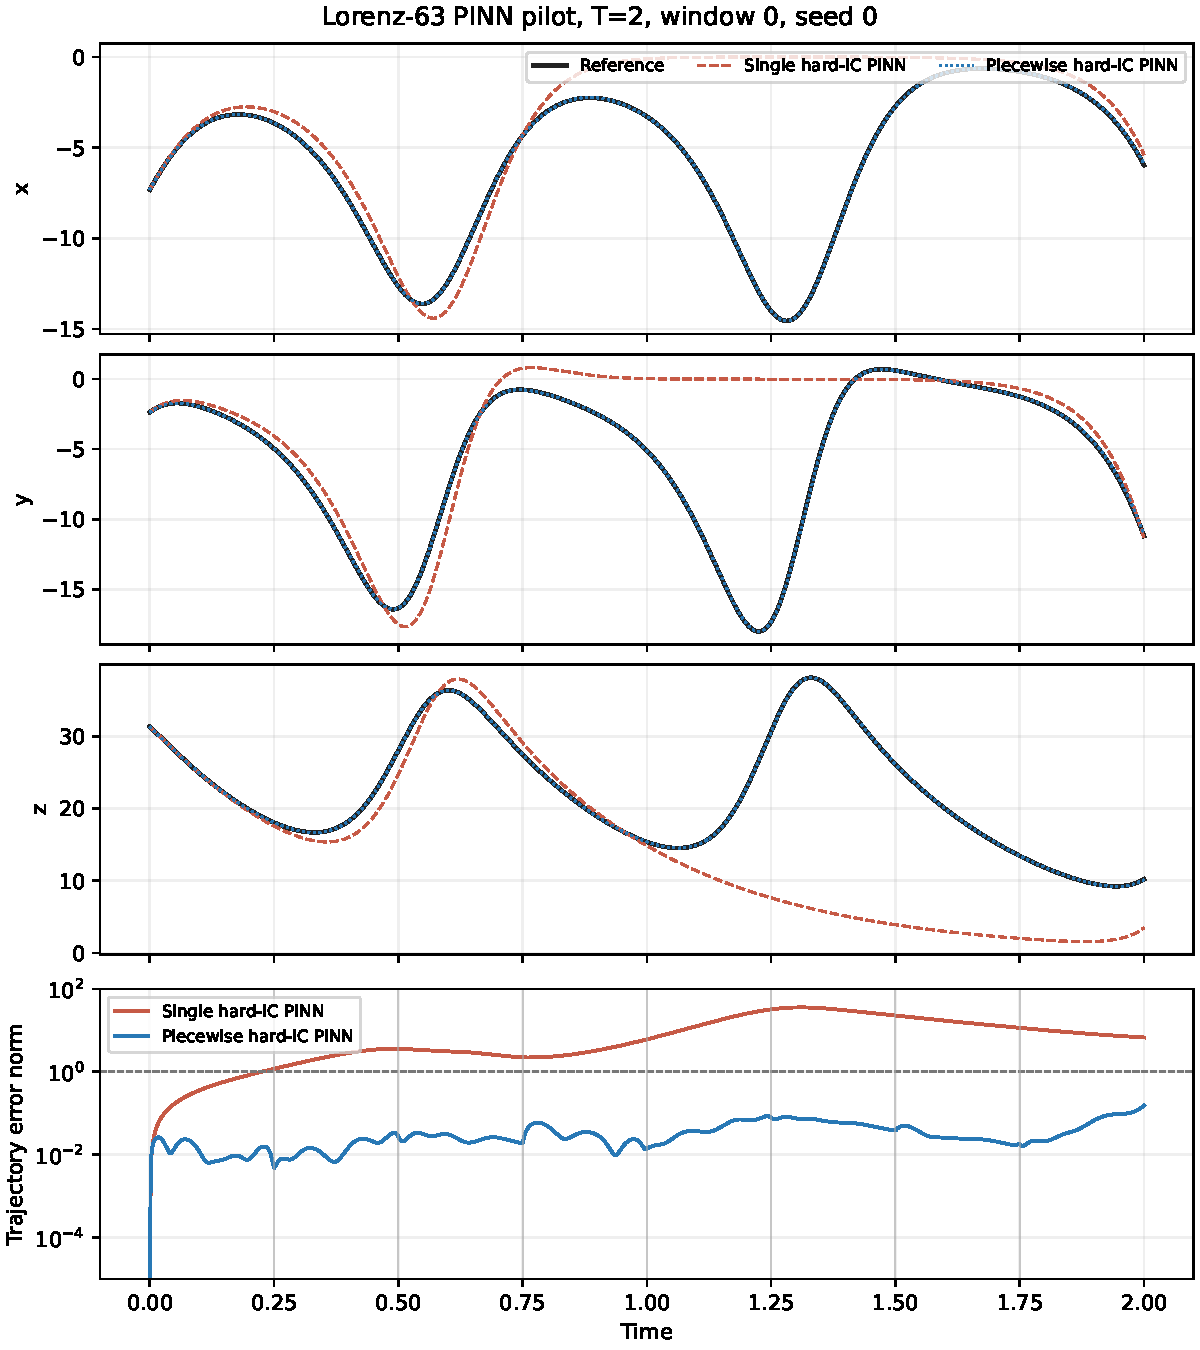
\includegraphics[width=.83\linewidth]{piecewise_pinn_t2_pilot.pdf}
\caption{Pilot reference and sequential PINN over $T=2$, with trajectory-error panel. It demonstrates one successful initial condition, not population-wide reliability.}\label{fig:pilot}
\end{figure}

\subsection{Frozen fresh-window validation}
To check generalization after model development, we froze all segment, training, and analysis settings and generated a new long-run Lorenz trajectory starting from $(7,8,9)$ rather than $(1,1,1)$. Fresh windows 1--8 and seeds 0--4 gave 40 new finite runs, none omitted. The new reference passed 36/36 checks, and tangent quantities passed 31/31 checks. Median of run-level median trajectory errors was 0.0551, and median of run maxima was 0.3991. Crucially, \textbf{30/40} runs stayed below error 1 throughout $T=2$ and 32/40 did so for at least 90\% of the window. Full-window success counts across windows 1--8 were $(0,5,2,5,5,4,4,5)$ out of five. The method is substantially better than the global pilot, but failures cluster by initial condition; the development-set 35/40 figure was optimistic for this new set \cite{validation}.
\begin{table}[H]\centering\small
\caption{Frozen fresh-reference run log, five seeds per window. The window median is the median of five run-level median errors; worst maximum is the largest error reached by any seed. A small median can coexist with late failure.}\label{tab:freshwindows}
\begin{tabular}{@{}cccc@{}}\toprule
Window & Median of run medians & Worst maximum & Runs with $E(t)<1$ throughout\\\midrule
1 & 0.0187 & 5.692 & 0/5\\
2 & 0.0636 & 0.511 & 5/5\\
3 & 0.0374 & 2.626 & 2/5\\
4 & 0.0741 & 0.316 & 5/5\\
5 & 0.0436 & 0.177 & 5/5\\
6 & 0.0995 & 1.149 & 4/5\\
7 & 0.0656 & 1.559 & 4/5\\
8 & 0.0630 & 0.168 & 5/5\\\bottomrule
\end{tabular}
\end{table}
Window 1 illustrates why we report maxima and full-window success as well as medians: all five runs cross error 1 at some time even though their median run error is low. A model can track much of a chaotic trajectory and still fail near the end. The eight windows, rather than the 40 seeded trainings or thousands of time samples, are the independent initial-condition units for uncertainty about transfer across trajectories. This is why the fresh oracle sensitivity resamples whole windows. The reference trust horizon remains longer than $T=2$, so these late discrepancies cannot be explained by the numerical reference reaching its documented accuracy limit.
\begin{figure}[H]\centering
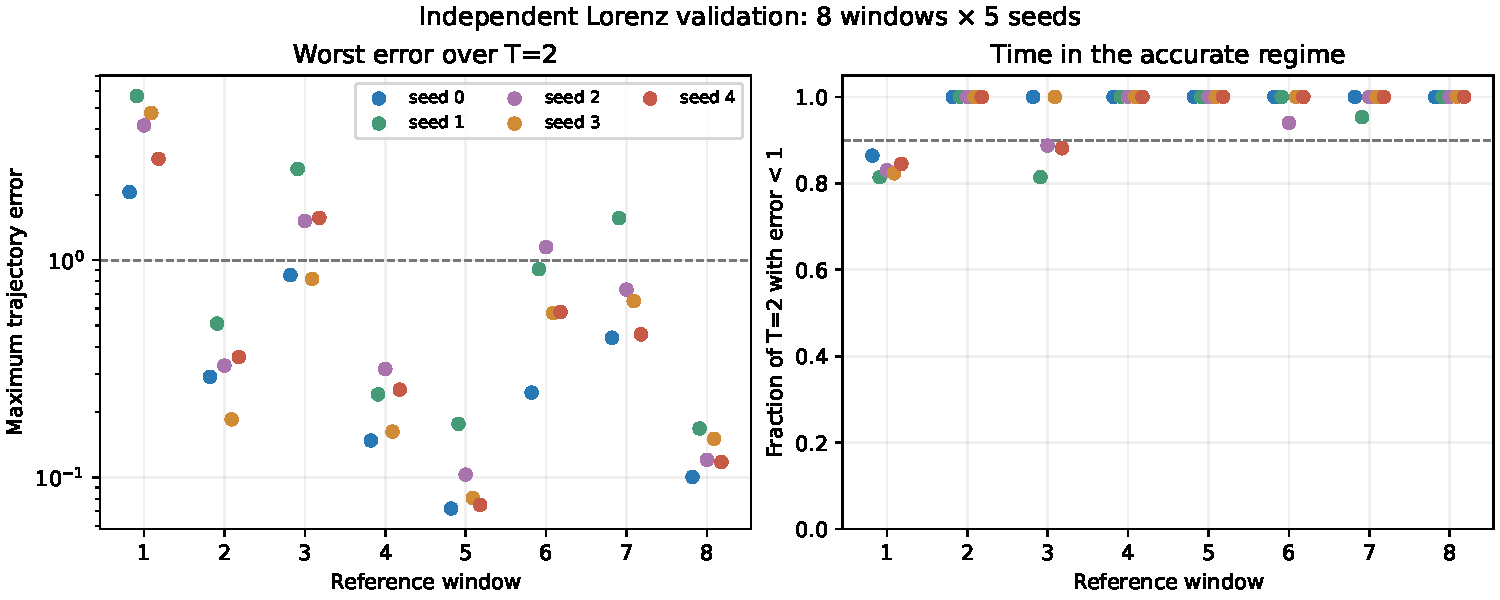
\includegraphics[width=.86\linewidth]{independent_validation_40runs.pdf}
\caption{All 40 frozen-model runs on the new eight initial conditions. Failures are included in the summary.}\label{fig:fresh}
\end{figure}

The unchanged directional analysis used 31,360 valid predictor samples after removing exact joins. Table~\ref{tab:fresh} shows that one-vector alignment again adds essentially no held-out predictive value. Neither $b_1$ nor $s_1$ passes the original four-part rule at any of the five horizons. Restricting to samples whose current and future error are both below 1 gives the same verdict (29,933 samples). Thus poor trajectories alone do not explain the original null result.
\begin{table}[H]\centering\small
\caption{Frozen fresh-window sequential PINNs: residual-only pooled held-out $R^2$ and feature gains. All 40 runs are included.}\label{tab:fresh}
\begin{tabular}{@{}ccccc@{}}\toprule
$\Delta$ & $R^2(M_0)$ & $\Delta R^2(b_1)$ & $\Delta R^2(s_1)$ & $\Delta R^2(\Phi)$\\\midrule
0.05 & $-.005$ & $-.0018$ & $-.0016$ & $+.0005$\\
0.10 & $-.005$ & $-.0009$ & $-.0003$ & $+.0068$\\
0.25 & $+.001$ & $-.0043$ & $-.0003$ & $+.0664$\\
0.50 & $-.021$ & $+.0062$ & $-.0079$ & $+.2672$\\
1.00 & $-.061$ & $-.0009$ & $-.0034$ & $+.3691$\\\bottomrule
\end{tabular}
\end{table}
The raw residual-only $R^2$ is near zero or negative, consistent with the target's inherited-error component. A separate, post-hoc sensitivity analysis therefore adds elapsed time and time squared to the residual-magnitude baseline and resamples whole initial-condition windows, keeping each window's five seeds together. The \emph{oracle} full-amplification gain beyond that baseline is $+0.056$ with window-bootstrap interval $[0.031,0.083]$ at $\Delta=0.25$; $+0.258$ $[0.206,0.395]$ at $0.5$; and $+0.442$ $[0.267,0.672]$ at $1.0$. The single-direction features still do not show useful positive gains. These intervals describe eight-window uncertainty for a secondary, reference-dependent feature, not a new practical predictor or causal training result \cite{validation}.

\section{Direct test of the paper's adaptive time weighting}\label{sec:adaptive}
After the first version of this report, we cloned the author's official code at commit \texttt{0595f4c} \cite{authorcode}. Its Lorenz implementation uses a fixed time grid and updates normalized residual-loss weights from the current candidate trajectory after every training epoch. We ported that rule to the existing PyTorch trainer so it could be tested under our architecture and reference protocol. At fixed grid times $t_i=iT/(N-1)$, the discrete rate proxy and weights are
\begin{align}\label{eq:adaptiveactual}
\widehat\lambda_i&=\frac{f(\widehat X_\theta(t_i))^\top\widehat X_\theta(t_i)}
{\norm{\widehat X_\theta(t_i)}^2+10^{-10}},\qquad \delta t=\frac{T}{N-1},\\
q_i&=\frac{\exp[-\delta t\sum_{j=0}^i\widehat\lambda_j]}
{\sum_k\exp[-\delta t\sum_{j=0}^k\widehat\lambda_j]},\qquad
L_{\rm adaptive}=\sum_i q_i\norm{r(t_i)}^2.
\end{align}
The weights are updated from the network after each Adam step and held fixed during the next gradient calculation. The initial condition is enforced exactly. Equation~\eqref{eq:adaptiveactual} implements the paper's Eq.~\eqref{eq:rho} and practical proxy Eq.~\eqref{eq:lambdaest} in physical time. The author's Lorenz code instead uses $\delta t_{\rm code}=1/(N-1)$ in its cumulative sum even for its $T=0.5$ interval. We tested that literal scaling as a separate \texttt{turinici\_code} mode, changing only $\delta t$. Our weighted objective is normalized to the same scale as our uniform control; the author's TensorFlow loss has its own overall scaling. The author's complete architecture and schedule were not reproduced, so these are tests of its \emph{adaptive weighting rule within our PINN}, not a reproduction of every published numerical result.

To isolate weighting, each adaptive run has a uniform-weight control with the same fixed grid, hard-IC model, seed, updates, and optimizer. In the global $T=2$ window-0 pilot, both used 20,000 updates and 256 collocation points. Uniform weights gave median trajectory error 17.473 and error below 1 for 3.20\% of the interval; adaptive weights gave 17.415 and 4.10\%. Both failed to solve the full trajectory. The adaptive run's final weights put 74.1\% of their mass on the last quarter of the grid and only 1.34\% on the first quarter; their max/min ratio was about 202. Its final \emph{weighted} training loss was smaller, but that is a different objective from the uniform loss and did not establish trajectory improvement.

Because the paper's own Lorenz experiments use shorter intervals, we also tested the rule within eight consecutive $0.25$-unit segments. The matched window-0 pilot used 4000 updates and 256 fixed points per segment. Uniform weighting gave median error 0.03594 and maximum 0.3130; adaptive weighting gave median 0.04203 and maximum 0.4094. Both stayed below error 1 throughout. Final weight contrasts on these short segments ranged from about 1.4 to 2.3, much nearer uniform than the global weights.

We then ran the same pair on all eight original analysis starting conditions at seed 0, without selecting only favorable windows. Table~\ref{tab:adaptive} reports trajectory error against the trusted reference, which is the common outcome for both objectives. The median of run-level median errors was 0.04326 with uniform weights and 0.04666 with adaptive weights. The adaptive run had a lower median error in only one of eight paired windows. Both methods stayed below error 1 throughout on seven of eight windows; both failed late on window 1. Mean training time per two-unit run was 88.2 versus 96.9 seconds, respectively. Thus this port of the paper's rule did not improve our sequential PINN in this one-seed comparison. The source code, all run files, and the comparison protocol are recorded in \cite{adaptiveprogress}.
\begin{table}[H]\centering\small
\caption{Matched fixed-grid sequential PINNs, seed 0: per-window median and maximum Euclidean trajectory errors. Only time weighting differs within a row.}\label{tab:adaptive}
\begin{tabular}{@{}ccccc@{}}\toprule
Window & Uniform median & Adaptive median & Uniform maximum & Adaptive maximum\\\midrule
1 & 0.04474 & 0.04331 & 7.3613 & 7.6281\\
2 & 0.05781 & 0.06783 & 0.4514 & 0.5184\\
3 & 0.04615 & 0.05122 & 0.1962 & 0.2536\\
4 & 0.02412 & 0.02437 & 0.0843 & 0.1050\\
5 & 0.04291 & 0.05001 & 0.1492 & 0.1604\\
6 & 0.04362 & 0.05260 & 0.2637 & 0.3181\\
7 & 0.02612 & 0.02718 & 0.0672 & 0.0685\\
8 & 0.03860 & 0.04294 & 0.1398 & 0.1695\\\bottomrule
\end{tabular}
\end{table}
These are eight starting conditions already used during model development, with one seed each. They are descriptive follow-up evidence, not a fresh 40-run validation or a reproduction of the paper's published TensorFlow comparison. The rate proxy in Eq.~\eqref{eq:adaptiveactual} is not guaranteed to equal the one-sided bound rate required in Eq.~\eqref{eq:onesided}; the global pilot's strong late weighting illustrates that gap. The observed sequential advantage is still attributable to the complete segmented training package, not to this adaptive weighting option.

The literal source-code time scale produced a different, stronger weighting distribution on short segments. Its matched global $T=2$ pilot still failed (median error 17.489 versus 17.473 uniform). On the eight sequential windows, the median of run-level median errors was 0.10283, versus 0.04326 uniform and 0.04666 with Eq.~\eqref{eq:adaptiveactual}'s physical-time scale. It lowered median error on 0/8 windows and stayed below error 1 throughout on 6/8, versus 7/8 for each other method. Table~\ref{tab:codeweights} gives all eight outcomes. This source-code scaling is a sensitivity to the published implementation, not a separate theorem or an independent validation set.
\begin{table}[H]\centering\small
\caption{Literal author-code cumulative time scale, same eight fixed-grid sequential windows and seed 0 as Table~\ref{tab:adaptive}. Values are Euclidean trajectory errors.}\label{tab:codeweights}
\begin{tabular}{@{}ccc@{}}\toprule
Window & Source-scale median & Source-scale maximum\\\midrule
1 & 0.13425 & 36.8641\\
2 & 0.13275 & 0.8259\\
3 & 0.09457 & 0.5071\\
4 & 0.07770 & 0.4043\\
5 & 0.09132 & 0.3598\\
6 & 0.23774 & 1.4802\\
7 & 0.05422 & 0.1138\\
8 & 0.11110 & 0.4789\\\bottomrule
\end{tabular}
\end{table}
\begin{figure}[H]\centering
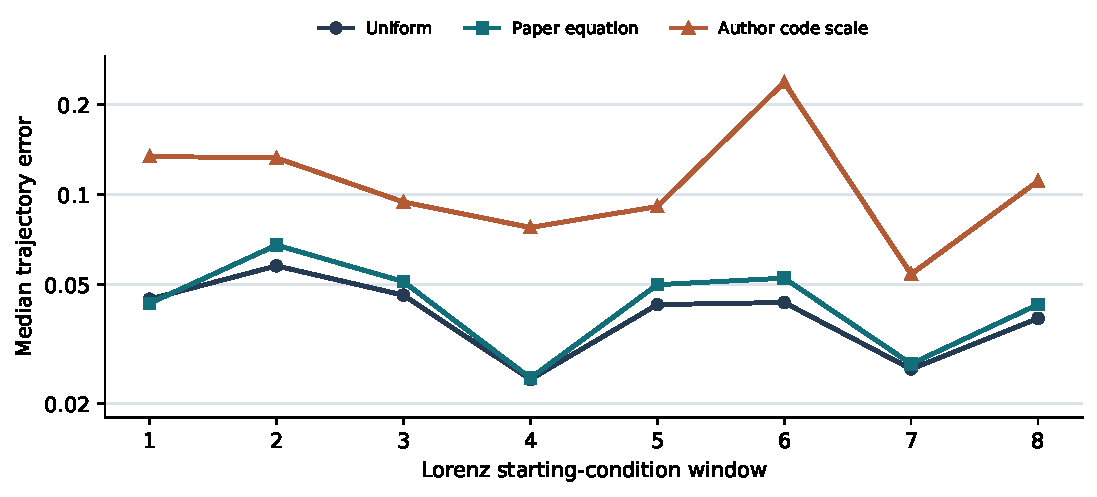
\includegraphics[width=.82\linewidth]{report_adaptive_paired_windows.pdf}
\caption{Matched fixed-grid sequential trainings on the eight previously used analysis windows, seed 0. The vertical axis is logarithmic; lower median trajectory error is better. ``Paper equation'' uses physical-time spacing in the density, while ``author code scale'' uses the time step in the released Lorenz script. This is an exploratory within-architecture comparison, not the paper's published benchmark.}\label{fig:adaptivepaired}
\end{figure}
The code-scale result does not contradict the paper's minimax statement: that statement assumes a suitable scalar growth bound and a fixed weighted-residual budget, whereas this is finite neural-network optimization with a rough state/zero rate proxy. It does show that neither implemented scaling was a demonstrated trajectory improvement for our Lorenz solver in the matched tests \cite{adaptiveprogress}.

\section{Final conclusion and limits}
The original goal was to learn whether the orientation of a PINN's local ODE violation could improve forecasts of its future error. The mathematical motivation is sound: for equal-size defects, linear dynamics can amplify one direction and damp another. The original empirical hypothesis, however, was \textbf{not supported}: neither backward Lyapunov alignment nor leading finite-time singular alignment improves held-out prediction enough to meet the fixed rule in the initial standard-PINN study or the frozen fresh-window sequential-PINN study. This is a Lorenz-63, architecture- and task-specific conclusion, not a theorem that direction never matters.

The research also identified what was more useful in these data. Recent residual \emph{history} predicts short-horizon total error in an exploratory sparse-sampling study, while the full tangent propagator's amplification of all residual components carries reference-dependent information at longer horizons. The latter cannot be deployed as measured here because it requires the true trajectory. Sequential hard-IC training extended useful trajectories from the original $T=1$ limit to $T=2$ for most new runs; its observed full-window success rate was 30/40, so the model remains sensitive to initial condition. Fixed early weighting and L-BFGS refinement did not materially improve their global pilots. Neither tested time scale of the ported Turinici adaptive rule improved the matched global pilot or the eight-window, one-seed sequential comparison. No Gaussian-process smoother, held-out Duhamel-integral regressor, or directional loss has been claimed as a completed result.

The main limitations are eight initial-condition clusters per set, one chaotic system, one base architecture, post-hoc choices in the interpolation and model-improvement branches, and an oracle analysis that uses a trusted numerical reference. The fresh model was frozen before those new windows were evaluated, but its design followed the earlier results; this is an independent-initial-condition validation of a developed method, not a preregistered independent method discovery. A future practical extension would estimate time-integrated amplification from the candidate trajectory and test it on new systems and new initial conditions. The present project reaches a defensible conclusion without claiming that unperformed extensions succeeded.

\appendix
\section{Reproducibility map}
\begingroup\small
The source repository provides the complete numerical record. Main checkpoints are:
\begin{itemize}\raggedright
\item Original plan and results: \path{docs/analysis_plan.md}, \path{docs/results.md}, \path{results/analysis/metrics.json}.
\item Baseline setup and theory checks: \path{docs/phase4_pinn.md}, \path{docs/phase2_lorenz_reference.md}, \path{docs/phase3_lyapunov.md}.
\item Interpolation protocol and output: \path{docs/interpolation_study.md}, \path{docs/interpolation_progress.md}, \path{results/interpolation_rebuild/interpolation_box_control/metrics.json}.
\item Model development and frozen validation: \path{docs/model_improvement_progress.md}, \path{docs/independent_validation_plan.md}, \path{docs/validation_progress_2026-11-22.md}, \path{results/independent_validation/}.
\item Adaptive weighting port and paired runs: \path{docs/adaptive_weighting_progress_2026-11-22.md}, \path{results/adaptive_time_weighting/sequential_seed0_summary.json}, \path{results/adaptive_time_weighting/sequential_code_seed0_summary.json}.
\end{itemize}
The experiment entry points are the numbered scripts 03, 04, 06, 07, 09, 13, 17, 20, 22, and 23 in \path{experiments/}. Script 23 regenerates Figures~\ref{fig:interpolation} and \ref{fig:adaptivepaired} from the saved JSON metrics. Large raw arrays are ignored by version control; the scripts and saved configurations specify how they were generated. The full automated suite had 131 passing tests after the adaptive port.
\endgroup

\begin{thebibliography}{9}
\bibitem{turinici} G. Turinici, ``Regime-Aware Time Weighting for Physics-Informed Neural Networks,'' arXiv:2407.21642v2 (2025), \url{https://arxiv.org/abs/2407.21642v2}. Local copy: \texttt{docs/2407.21642v2.pdf}.
\bibitem{submitted} Differential Equations project team, \emph{Project Report -- Differential Equations -- 2}, submitted report, local file \texttt{docs/Project Report - Differential Equations -2.pdf}.
\bibitem{phase0} Project record, \texttt{docs/phase0\_linear\_saddle.md} and \texttt{results/linear\_sanity/metrics.json}.
\bibitem{phase2} Project record, \path{docs/phase2_lorenz_reference.md} and \path{results/lorenz_reference/metrics.json}.
\bibitem{phase3} Project record, \texttt{docs/phase3\_lyapunov.md} and \texttt{results/lorenz\_lyapunov/metrics.json}.
\bibitem{phase4} Project record, \texttt{docs/phase4\_pinn.md}.
\bibitem{plan} Project record, \texttt{docs/analysis\_plan.md}, fixed before the original main analysis.
\bibitem{results} Project record, \texttt{docs/results.md} and \texttt{results/analysis/metrics.json}.
\bibitem{interpolation} Project record, \texttt{docs/interpolation\_study.md} and \texttt{docs/interpolation\_progress.md}.
\bibitem{modelprogress} Project record, \texttt{docs/model\_improvement\_progress.md}.
\bibitem{validation} Project record, \path{docs/independent_validation_plan.md} and \path{docs/validation_progress_2026-11-22.md}.
\bibitem{authorcode} G. Turinici, official code for the reference paper, commit \texttt{0595f4c}, \url{https://github.com/gabriel-turinici/physics_informed_neural_networks_time_sampling}.
\bibitem{adaptiveprogress} Project record, \path{docs/adaptive_weighting_progress_2026-11-22.md} and \path{results/adaptive_time_weighting/sequential_seed0_summary.json}.
\end{thebibliography}
\end{document}
